\documentclass{article}

% NeurIPS 2025 style. [preprint] prints the author names without claiming acceptance at NeurIPS.
\PassOptionsToPackage{numbers, compress}{natbib}
\usepackage[preprint]{neurips_2025}

\usepackage[utf8]{inputenc}
\usepackage[T1]{fontenc}
\usepackage{hyperref}
\usepackage{url}
\usepackage{booktabs}
\usepackage{amsfonts}
\usepackage{amsmath}
\usepackage{nicefrac}
\usepackage{microtype}
\usepackage{xcolor}
\usepackage{graphicx}
\usepackage{multirow}
\usepackage{tikz}
\usetikzlibrary{positioning, arrows.meta, calc}

% Every number below comes from results/tables/macros.tex, written by run.py (src/report_assets.py)
% from the training logs, so the text cannot drift from the experiments.
\newcommand{\BenchDevice}{NVIDIA GeForce RTX 3060 Laptop GPU}
\newcommand{\LmiiMiou}{55.45}
\newcommand{\UnetMiou}{56.87}
\newcommand{\UnetPmMiou}{54.64}
\newcommand{\LmiiParams}{0.727}
\newcommand{\UnetParams}{1.927}
\newcommand{\UnetPmParams}{0.754}
\newcommand{\LmiiFps}{12.3}
\newcommand{\UnetFps}{109.5}
\newcommand{\UnetPmFps}{154.8}
\newcommand{\LmiiFpsG}{76.2}
\newcommand{\UnetFpsG}{107.6}
\newcommand{\UnetPmFpsG}{163.1}
\newcommand{\LmiiFpsGH}{115.4}
\newcommand{\UnetFpsGH}{170.7}
\newcommand{\UnetPmFpsGH}{255.5}
\newcommand{\LmiiTrainMin}{30}
\newcommand{\UnetTrainMin}{11}
\newcommand{\UnetPmTrainMin}{9}
\newcommand{\LmiiPeakGB}{4.32}
\newcommand{\LmiiGmacs}{4.99}
\newcommand{\UnetGmacs}{24.36}
\newcommand{\UnetPmGmacs}{9.57}
\newcommand{\PaperGap}{14.49}
\newcommand{\CcMean}{0.48}
\newcommand{\CcMin}{0.37}
\newcommand{\CcMax}{0.56}
\newcommand{\NumSeeds}{3}
\newcommand{\LmiiMiouHiRes}{48.06}
\newcommand{\LmiiFpsHiRes}{18.9}
\newcommand{\Epochs}{80}
\newcommand{\LmiiMiouSeedFortyTwo}{55.60}
\newcommand{\LmiiMiouStd}{0.58}
\newcommand{\UnetMiouStd}{0.55}
\newcommand{\UnetPmMiouStd}{0.38}


\newif\ifresultnotes\resultnotesfalse
\newcommand{\resultnote}[1]{\ifresultnotes{\color{blue!70!black}\textit{[#1]}}\fi}

% primitive \input, so generated table rows can be followed by \bottomrule inside a tabular
\makeatletter\newcommand{\tabinput}[1]{\@@input results/tables/#1.tex }\makeatother

\title{Lightweight Real-Time Semantic Segmentation:\\
Reproducing LMIINet's Efficiency and Accuracy on CamVid}

\author{%
  Prakhar Srivastava \\
  B23CM1056 \\
  Indian Institute of Technology Jodhpur \\
  \texttt{b23cm1056@iitj.ac.in} \\
  \And
  Neer Bipinkumar Modi \\
  B23CS1043 \\
  Indian Institute of Technology Jodhpur \\
  \texttt{b23cs1043@iitj.ac.in} \\
}

\begin{document}

\maketitle

\begin{abstract}
Real-time semantic segmentation has to balance accuracy against parameters, compute and measured
speed. LMIINet~\cite{qiu2024lmiinet} reports 69.94\% mIoU on CamVid with 0.72M parameters at
160\,FPS, obtained by letting the local and context branches of each block, and a linear-attention
Transformer and a channel-attention block, exchange learned and weighted copies of their outputs.
The paper has no public code. We rebuild LMIINet from its equations (\LmiiParams{}M parameters),
train it from scratch for \Epochs{} epochs, and compare it with a U-Net of the same depth and a
parameter-matched U-Net under one recipe and one timing protocol on a laptop RTX 3060. Over
\NumSeeds{} seeds LMIINet reaches \LmiiMiou\% test mIoU, against \UnetMiou\% for the U-Net with
2.6 times its parameters and \UnetPmMiou\% for the parameter-matched U-Net, a lead that is not statistically significant, while the larger
U-Net's lead over LMIINet is ($p = 0.04$). Ablations show that the
Transformer, the channel reconstruction unit and the feature-enhancement decoder each add one to
one and a half points, while the learned interaction coefficients, the paper's central idea, add
nothing at this scale. With half or a quarter of the training images the lead over the
parameter-matched U-Net disappears. Speed does not follow the MAC count: LMIINet needs a fifth of
U-Net's compute but runs slower on this GPU (\LmiiFpsG{} against \UnetFpsG{}\,FPS replayed as CUDA
graphs, and only \LmiiFps{}\,FPS in eager PyTorch), because its many small kernels are limited by
launch overhead and memory traffic rather than arithmetic.
Code: \url{https://github.com/CoPrime69/lmiinet-camvid}.
\end{abstract}

% =====================================================================
\section{Introduction}
\label{sec:intro}

Semantic segmentation assigns a class to every pixel. In driving and robotics it has to run at
frame rate on modest hardware, so a model is judged on accuracy together with parameters, compute
and measured speed. Encoder-decoders such as U-Net~\cite{ronneberger2015unet} and
SegNet~\cite{badrinarayanan2017segnet} are accurate but spend most of their compute on
full-resolution convolutions. Real-time networks (ENet~\cite{paszke2016enet},
ERFNet~\cite{romera2018erfnet}, BiSeNet~\cite{yu2018bisenet}) cut that cost with factorised and
dilated convolutions, and recent hybrids (MobileViT~\cite{mehta2022mobilevit},
TopFormer~\cite{zhang2022topformer}, LETNet~\cite{xu2023letnet}) add a Transformer for global context.

LMIINet~\cite{qiu2024lmiinet} reports a strong point on this trade-off: 0.72M parameters and
69.94\% mIoU at 160\,FPS on CamVid (RTX 2080Ti). Its central idea is \emph{multiple-information
interaction}. Instead of running a local path and a context path side by side and summing them,
each path receives a learned, weighted copy of the other's output, and the same device couples a
linear-attention Transformer to a channel-attention block. The paper has no public code, leaves
several design details open, and does not state its training schedule.

\paragraph{Contributions.} This project tests whether LMIINet's efficiency and accuracy advantage
holds when the model is rebuilt from the paper alone and trained at a much smaller scale
(Section~\ref{sec:problem} states the questions precisely). Our contributions are:
\begin{itemize}
  \item An independent PyTorch implementation of LMIINet with \LmiiParams{}M parameters (paper:
        0.72M). Every unspecified detail and our choice for it is listed in
        Appendix~\ref{app:decisions}, and the attention, metric and complexity code is checked
        against independent references (Appendix~\ref{app:tests}).
  \item A controlled comparison with a U-Net of the same depth and a parameter-matched U-Net,
        trained with one recipe and timed with one protocol on one GPU.
  \item Ablations of the components that carry the interaction idea, and a reduced-data study
        with 25\% and 50\% of the training images.
  \item A measurement of where the time goes when such a network runs on a laptop GPU, which
        turns out to matter as much for the efficiency claim as the parameter count does.
\end{itemize}

% =====================================================================
\section{Literature Review}
\label{sec:related}

\paragraph{Real-time segmentation.} ENet~\cite{paszke2016enet} introduced early down-sampling and
asymmetric bottlenecks; ERFNet~\cite{romera2018erfnet} used factorised residual $3{\times}1$ and
$1{\times}3$ convolutions; BiSeNet~\cite{yu2018bisenet} split spatial detail and context into two
paths. LETNet~\cite{xu2023letnet}, from the same group as LMIINet, combines a U-shaped CNN with a
Transformer at the bottleneck and long connections with feature enhancement. LMIINet keeps this
skeleton and replaces the blocks.

\paragraph{Efficient attention.} Softmax attention costs $\mathcal{O}(N^2d)$ for $N$ tokens.
Linear attention~\cite{katharopoulos2020transformers} replaces the softmax kernel with a feature map
$\phi$, so that $\phi(Q)(\phi(K)^\top V)$ costs $\mathcal{O}(Nd^2)$. FLatten
Transformer~\cite{han2023flatten} adds a \emph{focusing} function that sharpens the attention
distribution and a depthwise convolution that restores feature diversity. LMIINet builds its
global module on FLatten and couples it with the channel attention block (CAB) of
HAT~\cite{chen2023hat}.

\paragraph{Redundancy-reducing convolutions.} SCConv~\cite{li2023scconv} proposes a Channel
Reconstruction Unit (CRU) that splits the channels, transforms one part richly and reuses the
other cheaply. LMIINet places a CRU inside its bottleneck.

% =====================================================================
\section{Problem Statement}
\label{sec:problem}

\paragraph{Task.} Given an RGB road-scene image $I \in [0,255]^{H\times W\times 3}$, predict a label
map $\hat{Y} \in \{1,\dots,K\}^{H\times W}$ over the $K=11$ CamVid classes; pixels labelled
\emph{void} are ignored. Accuracy is the mean intersection-over-union over classes, accumulated over
the whole test set:
\begin{equation}
\mathrm{mIoU} = \frac{1}{K}\sum_{k=1}^{K}
\frac{\lvert\{\hat{Y}=k\}\cap\{Y=k\}\rvert}{\lvert\{\hat{Y}=k\}\cup\{Y=k\}\rvert}.
\end{equation}
Efficiency is measured by the number of parameters, the multiply-accumulates (MACs) per frame and
the frames per second (FPS) at batch size 1. A real-time segmentation network has to reach a high
mIoU while keeping all three small.

\paragraph{Claim under test.} LMIINet~\cite{qiu2024lmiinet} reports 69.94\% mIoU at 160\,FPS with
0.72M parameters on CamVid and attributes this to multiple-information interaction. The paper
releases no code and leaves its training schedule and several architectural details unspecified.

\paragraph{Research questions.} Rebuilding LMIINet from the paper alone and training it at a much
smaller scale than the paper, we ask:
\begin{enumerate}
  \item[RQ1] How close does an independent reimplementation come to the reported parameter count,
             accuracy and speed?
  \item[RQ2] Is it more accurate or faster than a U-Net of the same depth, and than a U-Net with the
             same number of parameters, when all three are trained and timed identically?
  \item[RQ3] Which of its components produce its accuracy, and in particular, does the learned
             interaction help?
  \item[RQ4] Does its advantage hold when less training data is available?
\end{enumerate}

\paragraph{Scope.} Every model is trained from scratch on one laptop GPU (RTX 3060, 6\,GB) for 80
epochs, a small fraction of the schedule used in related work, and evaluated on CamVid only.

% =====================================================================
\section{Proposed Method}
\label{sec:method}

To answer these questions we rebuild LMIINet from its equations (Figure~\ref{fig:arch},
Sections~\ref{sec:lfib} to \ref{sec:decoder}) and pair it with two U-Net baselines trained under
exactly the same conditions (Section~\ref{sec:baselines}).

\begin{figure}[t]
\centering
\resizebox{\textwidth}{!}{%
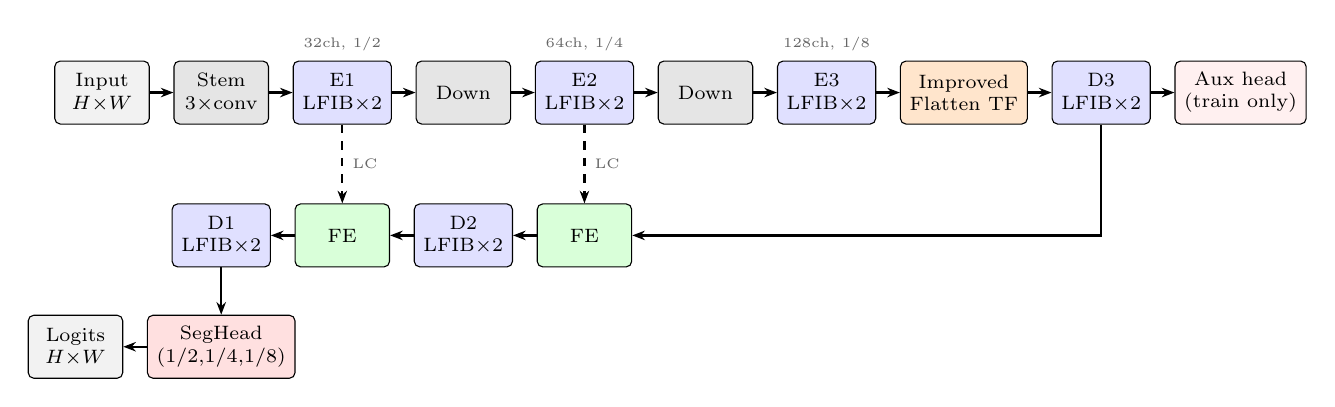
\begin{tikzpicture}[
  node distance=3mm,
  blk/.style={draw, rounded corners=2pt, minimum height=8mm, minimum width=12mm, align=center, font=\scriptsize, fill=#1},
  blk/.default=white,
  arr/.style={-{Stealth[length=1.6mm]}, thick},
  lab/.style={font=\tiny, text=black!60}]
  \node[blk=gray!10] (in) {Input\\$H{\times}W$};
  \node[blk=gray!20, right=of in] (stem) {Stem\\3$\times$conv};
  \node[blk=blue!12, right=of stem] (e1) {E1\\LFIB$\times$2};
  \node[blk=gray!20, right=of e1] (d1) {Down};
  \node[blk=blue!12, right=of d1] (e2) {E2\\LFIB$\times$2};
  \node[blk=gray!20, right=of e2] (d2) {Down};
  \node[blk=blue!12, right=of d2] (e3) {E3\\LFIB$\times$2};
  \node[blk=orange!20, right=of e3] (tf) {Improved\\Flatten TF};
  \node[blk=blue!12, right=of tf] (de3) {D3\\LFIB$\times$2};
  \node[blk=red!6, right=of de3] (aux) {Aux head\\(train only)};
  \node[blk=green!15, below=10mm of e2] (fe2) {FE};
  \node[blk=blue!12, left=of fe2] (de2) {D2\\LFIB$\times$2};
  \node[blk=green!15, below=10mm of e1] (fe1) {FE};
  \node[blk=blue!12, left=of fe1] (de1) {D1\\LFIB$\times$2};
  \node[blk=red!12, below=6mm of de1] (head) {SegHead\\(1/2,1/4,1/8)};
  \node[blk=gray!10, left=of head] (out) {Logits\\$H{\times}W$};
  \draw[arr] (in) -- (stem); \draw[arr] (stem) -- (e1); \draw[arr] (e1) -- (d1); \draw[arr] (d1) -- (e2);
  \draw[arr] (e2) -- (d2); \draw[arr] (d2) -- (e3); \draw[arr] (e3) -- (tf); \draw[arr] (tf) -- (de3);
  \draw[arr] (de3) -- (aux);
  \draw[arr] (de3.south) |- (fe2.east);
  \draw[arr, dashed] (e2) -- node[lab, right]{LC} (fe2);
  \draw[arr] (fe2) -- (de2);
  \draw[arr] (de2) -- (fe1);
  \draw[arr, dashed] (e1) -- node[lab, right]{LC} (fe1);
  \draw[arr] (fe1) -- (de1);
  \draw[arr] (de1) -- (head); \draw[arr] (head) -- (out);
  \node[lab, above=0mm of e1] {32ch, 1/2}; \node[lab, above=0mm of e2] {64ch, 1/4};
  \node[lab, above=0mm of e3] {128ch, 1/8};
\end{tikzpicture}}
\caption{LMIINet as reimplemented. Six LFIB stages of two blocks each (the paper's
\{2,2,2,2,2,2\} setting), one improved Flatten Transformer block at 1/8 resolution, two long
connections (LC) feeding encoder detail into feature-enhancement (FE) modules, a SegHead fusing
the 1/2, 1/4 and 1/8 decoder outputs, and an auxiliary head at 1/8 used only in training.}
\label{fig:arch}
\end{figure}

\subsection{Lightweight Feature Interaction Bottleneck (LFIB)}
\label{sec:lfib}
Given $x\in\mathbb{R}^{C\times H\times W}$, LFIB applies a $1{\times}1$ convolution and splits the
result into two halves. A left branch of asymmetric $3{\times}1$ and $1{\times}3$ convolutions models
local structure; a right branch of a dilated depthwise $3{\times}3$ and a pointwise convolution
models context. The branches interact through combination coefficients (CC) $\alpha$, learnable
scalars initialised to $0.5$:
\begin{align}
F_1 &= H_{1\times1}(x), \qquad [F_{21}, F_{22}] = \mathrm{Split}(F_1),\\
F_{21}' &= H_{1\times3}\big(H_{3\times1}(F_{21} + \alpha_l F_{22})\big),\qquad
F_{22}' = H_{1\times1}\big(H^{d}_{3\times3,\mathrm{DW}}(F_{22} + \alpha_r F_{21}')\big),\\
F_2 &= [F_{21}', F_{22}'] + \mathrm{CRU}(F_1), \qquad
y = \mathrm{Shuffle}\big(H_{3\times3,\mathrm{DW}}(x + F_2)\big).
\end{align}
The CRU~\cite{li2023scconv} adds a cheap channel-reconstruction path and channel shuffle mixes the
two halves before the next block. Dilation rates grow with depth: (1,2), (2,4), (4,8) in the
encoder and (4,2), (2,1), (1,1) in the decoder.

\subsection{Improved Flatten Transformer}
At 1/8 resolution ($45{\times}60$ tokens for a $360{\times}480$ input) one Transformer block adds
global context through focused linear attention (FLAM)~\cite{han2023flatten}:
\begin{equation}
\phi_p(x) = \frac{\lVert x\rVert}{\lVert x^{p}\rVert}\,x^{p},\; x\leftarrow\mathrm{ReLU}(x),\qquad
\mathrm{FLAM}(X) = \mathrm{diag}(Z)\,\phi_p(Q)\big(\phi_p(K)^\top V\big) + \mathrm{DWC}(V),
\end{equation}
with focusing power $p=3$, 4 heads, a $5{\times}5$ depthwise convolution and
$Z_i = 1/(\phi_p(Q_i)^\top \sum_j \phi_p(K_j))$. Computing $\phi_p(K)^\top V$ first never forms the
$N{\times}N$ matrix. LMIINet couples the attention output to a CAB (two $3{\times}3$ convolutions
with GELU and channel attention~\cite{chen2023hat}) through a second combination coefficient:
\begin{align}
F_{11} &= \mathrm{FLAM}(\mathrm{LN}(x_t)),\qquad F_{12} = \mathrm{CAB}(x_t + \alpha_t F_{11}),\\
F_1 &= F_{11} + F_{12} + x_t, \qquad y_t = F_1 + \mathrm{MLP}(\mathrm{LN}(F_1)).
\end{align}
The power and normalisation steps run in fp32 even under mixed precision, since $x^{p}$ overflows
easily in 16-bit formats.

\subsection{Decoder, segmentation head and loss}
\label{sec:decoder}
Each decoder stage reduces and up-samples the deeper feature, and a feature-enhancement (FE)
module fuses it with the encoder feature carried by a long connection. FE gates the detail
feature with a spatial attention map computed from the semantic feature (CBAM
style~\cite{woo2018cbam}), adds the two, and refines the sum with a depthwise convolution and
ECA~\cite{wang2020eca}. The SegHead up-samples the 1/4 and 1/8 decoder outputs to 1/2,
concatenates them with the 1/2 output, and applies two $1{\times}1$ convolutions. Training
minimises $\mathcal{L} = \mathcal{L}_{\text{main}} + 0.3\,\mathcal{L}_{\text{aux}}$, both
class-weighted cross-entropy, with the auxiliary logits predicted directly from the 1/8 decoder
feature.

\subsection{Baselines}
\label{sec:baselines}
LMIINet bottoms out at 1/8 resolution, so our U-Net~\cite{ronneberger2015unet} uses three
down-sampling steps (four levels) of double $3{\times}3$ conv, BN and ReLU blocks with
transposed-convolution up-sampling. \textbf{U-Net} (base width 32, \UnetParams{}M parameters) is the
standard model of similar depth named in our proposal. \textbf{U-Net-PM} (base width 20,
\UnetPmParams{}M) has the same parameter budget as LMIINet, which separates the effect of the
architecture from the effect of size.

% =====================================================================
\section{Experiments and Results}
\label{sec:results}

\subsection{Experimental setup}
\label{sec:setup}

\paragraph{Data.} The 11-class CamVid split of SegNet~\cite{badrinarayanan2017segnet}: 367 training,
101 validation and 233 test images at $360{\times}480$, with the \emph{void} label ignored.

\paragraph{Training.} All models share the paper's CamVid recipe~\cite{qiu2024lmiinet}:
Adam~\cite{kingma2015adam} with $\beta_1=0.9$, initial learning rate $10^{-3}$, weight decay
$2{\times}10^{-4}$, batch size 8 and poly decay $(1-\text{iter}/\text{max\_iter})^{0.9}$
\cite{chen2018deeplab}. The paper does not report its schedule or augmentation. We train for
\Epochs{} epochs (3,600 iterations), from random initialisation, with random scaling in
$[0.75, 1.75]$, $360{\times}480$ crops, horizontal flips and mild colour jitter. Cross-entropy is
weighted with ENet weights $w_k = 1/\ln(1.02 + p_k)$~\cite{paszke2016enet}. We keep the checkpoint
with the best validation mIoU (evaluated every 5 epochs) and evaluate it once on the test set.
Training uses bf16 autocast.

\paragraph{Reduced-data study.} LMIINet and U-Net-PM are retrained on a fixed random 25\% and
50\% subset of the training images (the same subset for both models). The number of optimisation
steps is held at about 3,600 by scaling the epochs (3,520 to 3,680, as the subset sizes are not
multiples of the batch), so the comparison isolates the amount of data
rather than the amount of training.

\paragraph{Efficiency.} Parameters are counted exactly. MACs are counted for one
$360{\times}480$ image over convolutions, linear layers and the attention products; most
segmentation papers report this quantity as ``FLOPs''. FPS is measured at batch size 1 after a
warm-up, with the GPU synchronised before the clock is read, in two ways: eager PyTorch, and with
the forward pass captured once as a CUDA graph and replayed. All timings come from one laptop
RTX 3060 (6\,GB) under Windows, so they compare with each other but not with the paper's 2080Ti.

% =====================================================================
\begin{table}[t]
\caption{CamVid test set at $360{\times}480$. FPS at batch 1 on \BenchDevice{}, in eager PyTorch
and as a CUDA-graph replay (fp32 and fp16). The last row is the paper's reported result on an RTX
2080Ti after a longer, unstated schedule (n/r: not reported).}
\label{tab:main}
\centering
\small
\setlength{\tabcolsep}{4pt}
\resizebox{\textwidth}{!}{%
\begin{tabular}{lccccccc}
\toprule
 & & & \multicolumn{3}{c}{FPS} & & \\
\cmidrule(lr){4-6}
Model & Params (M) & GMACs & eager & graph & graph fp16 & mIoU (\%) & Pixel acc. (\%) \\
\midrule
\tabinput{main_table}
\bottomrule
\end{tabular}}
\end{table}

\begin{figure}[t]
\centering
\begin{minipage}{0.49\textwidth}\centering
  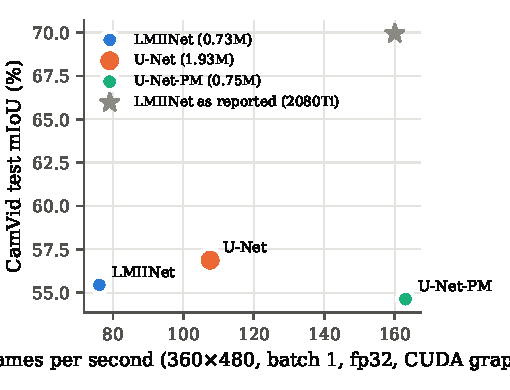
\includegraphics[width=\linewidth]{figures/01_miou_vs_fps.pdf}
\end{minipage}\hfill
\begin{minipage}{0.49\textwidth}\centering
  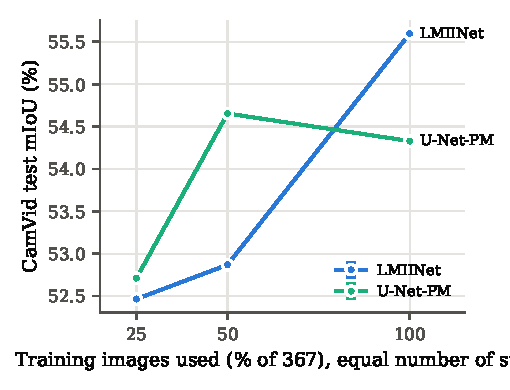
\includegraphics[width=\linewidth]{figures/02_data_scale.pdf}
\end{minipage}
\caption{\textbf{Left:} test mIoU against speed (CUDA-graph replay, fp32; marker area grows with
the parameter count; star: the paper's reported point on a different GPU). \textbf{Right:} test mIoU
against the share of training images used, at an equal number of optimisation steps.}
\label{fig:tradeoff}
\end{figure}

\subsection{Accuracy, size and speed}
Table~\ref{tab:main} gives the main comparison, as the mean and standard deviation over
\NumSeeds{} seeds. LMIINet reaches \LmiiMiou{} $\pm$ \LmiiMiouStd\% test mIoU with \LmiiParams{}M
parameters and \LmiiGmacs{} GMACs per frame. The parameter-matched U-Net-PM reaches \UnetPmMiou{}
$\pm$ \UnetPmMiouStd\% with almost the same parameter count and twice the compute, and the standard
U-Net reaches \UnetMiou{} $\pm$ \UnetMiouStd\% with 2.6 times the parameters and five times the
compute. Ranked by the mean, the standard U-Net is first, LMIINet second and U-Net-PM third. The U-Net
is ahead of LMIINet in every seed, by 0.5 to 1.9 points. LMIINet's lead over the parameter-matched
U-Net is smaller and less certain: it is ahead by 1.3 and 1.4 points in two seeds and behind by 0.3
in the third, a mean of 0.8 points against seed-to-seed standard deviations of 0.4 to 0.6. Welch's
$t$-test on the three seeds separates U-Net from LMIINet ($p = 0.04$) but not LMIINet from U-Net-PM
($p = 0.12$). At the paper's 0.72M budget LMIINet is therefore on par with a plain U-Net of the
same size, which needs about twice its MACs but, as the next section shows, runs twice as fast.

LMIINet is \PaperGap{} points below the paper's 69.94\%. We attribute most of the gap to the
training schedule. Without a long run this cannot be proven, but three observations from our logs
point the same way. First, no model had converged: all nine runs of the main comparison reached
their best validation score within the last fifteen of their 80 epochs, and in every one of them
the mean training loss over epochs 71 to 80 is still below that over epochs 61 to 70. Second, the
gap in training is large: related work from the same group trains CamVid for about 1000
epochs~\cite{xu2023letnet}, roughly 45,000 updates at batch 8 against our 3,600, a factor of
about twelve. Third, on this split the test set is markedly harder than the validation set: best
validation mIoU is 7 to 12 points above test mIoU for every model and largest for LMIINet (about
67\% against 56\%), so a checkpoint chosen on validation does not carry its score over to test.
Several architectural details are also our own choices (Appendix~\ref{app:decisions}) and could
account for part of the remainder. The decisive test is a single LMIINet run of 300 to 1000
epochs with the code as released.

\subsection{Where the time goes on a laptop GPU}
LMIINet needs \LmiiGmacs{} GMACs per $360{\times}480$ frame, against \UnetGmacs{} for U-Net and
\UnetPmGmacs{} for U-Net-PM, so on paper it should be the fastest of the three by a wide margin.
On our laptop GPU it is the slowest (Table~\ref{tab:main}). Two separate effects are at work.

The first is launch overhead. In eager PyTorch every operation is a separate kernel launched from
Python, and LMIINet's forward pass consists of several hundred small ones (each of the twelve LFIBs launches about
forty, counting normalisation, activation, the CRU and the channel shuffle). Its eager speed is \LmiiFps{}\,FPS, while replaying
the same forward pass as a captured CUDA graph, which issues the identical kernels without the
per-launch cost, gives \LmiiFpsG{}\,FPS. For U-Net, which has few and large kernels, the two
figures are almost equal (\UnetFps{} and \UnetFpsG{}\,FPS). In eager mode LMIINet is therefore
bound by the CPU, not the GPU.

The second is memory traffic. Even as a CUDA graph LMIINet stays behind both U-Nets
(\LmiiFpsG{} against \UnetFpsG{} and \UnetPmFpsG{}\,FPS in fp32, \LmiiFpsGH{} against \UnetFpsGH{}
and \UnetPmFpsGH{}\,FPS in fp16). Depthwise, asymmetric and $1{\times}1$ convolutions on 32 to 128
channels do little arithmetic per byte they read, and each LFIB also splits, concatenates, shuffles
and re-normalises its feature maps. Those operations cost memory bandwidth and appear in no MAC
count. The same property shows in training: LMIINet's peak training memory at batch 8 is
\LmiiPeakGB{}\,GB in bf16, more than either U-Net despite the smallest parameter count, and in fp32
it exceeded the 6\,GB card, at which point the Windows driver silently spilled into system memory
and every kernel ran 50 to 100 times slower.

None of this contradicts the paper's 160\,FPS, which was measured on a different GPU with an
unstated runtime. It does show that parameters and MACs are weak predictors of speed for this
kind of network, and that a speed claim needs the hardware, precision and execution mode next to
it.

\subsection{Ablation of the interaction mechanisms}

\begin{table}[t]
\caption{Ablations of LMIINet on CamVid test, same recipe and seed. $\Delta$ is the change in mIoU
against the full model.}
\label{tab:ablation}
\centering
\small
\begin{tabular}{lcccc}
\toprule
Variant & Params (M) & GMACs & mIoU (\%) & $\Delta$ \\
\midrule
\tabinput{ablation_table}
\bottomrule
\end{tabular}
\end{table}

Table~\ref{tab:ablation} removes one component at a time (seed 42 for every row, including the
full model, which scores \LmiiMiouSeedFortyTwo\% in that run). Three components earn their place.
Without the Flatten Transformer the network loses 1.0 point, without the CRU 1.0 point, and without
the feature-enhancement fusion 1.5 points. The first two are also the expensive ones: they hold 29\%
and 22\% of the parameters, and removing the CRU alone raises the CUDA-graph frame rate from 76 to
104\,FPS, the largest speed gain of any ablation.

The combination coefficients behave differently. Setting them to zero, which removes every
cross-branch and attention-to-CAB exchange while keeping the architecture and the parameter count
unchanged, gives 56.24\%, slightly \emph{above} the full model. In the full model the learned
coefficients end between \CcMin{} and \CcMax{} (mean \CcMean) after starting at 0.5, so training
barely uses the freedom it is given. At our scale, then, the multiple-information interaction that
gives LMIINet its name contributes nothing measurable; what helps is the set of components around
it.

\paragraph{How reliable are single-seed ablations?} Each ablation was trained once, so we judge it
against the spread of the full model over its three seeds ($55.45 \pm 0.58$). All four ablations
fall outside the range of those three runs: the three removals below the lowest of them and the
no-CC run above the highest. None, however, differs from the full model by more than about two
standard deviations, and with three reference runs a two-sided $t$-test on a single new run gives
$p$ between 0.19 and 0.36. The ablations therefore show a consistent direction (every removal
hurts, removing the coefficients does not) rather than a measured effect size, and a gain of 0.8
points without the coefficients should be read as ``no detectable benefit'', not as harm.

\paragraph{Why the coefficients can add little.} There is also a structural reason. In an LFIB the
halves $F_{21}$ and $F_{22}$ are two slices of one tensor $F_1 = H_{1\times1}(x)$. Adding
$\alpha_l F_{22}$ to the left branch feeds its $3{\times}1$ convolution a fixed linear mix of channels
that the learnable $1{\times}1$ convolution could nearly have placed in $F_{21}$ itself, so this
injection is close to a reparametrisation rather than new capacity. The right-hand injection does
carry something new, the processed left output, but the same exchange happens one step later in
any case: the halves are concatenated, added to the CRU output that sees all channels, mixed by the
channel shuffle, and passed to the next block's $1{\times}1$ convolution, which combines every
channel of both branches. The coefficients move this exchange a layer earlier rather than creating
it. The learned values agree: over the 75 coefficients of the three seeds the mean move away from
the initial 0.5 is 0.04 and the largest is 0.13.

\subsection{Smaller training sets}

\begin{table}[t]
\caption{CamVid test mIoU (\%) when training on a fixed random subset of the 367 training images,
with the number of optimisation steps held at about 3,600.}
\label{tab:scale}
\centering
\small
\begin{tabular}{lccc}
\toprule
Model & 25\% (92 images) & 50\% (184 images) & 100\% (367 images) \\
\midrule
\tabinput{scale_table}
\bottomrule
\end{tabular}
\end{table}

Table~\ref{tab:scale} and Figure~\ref{fig:tradeoff} (right) repeat the size-matched comparison with
less data, at the same number of optimisation steps. LMIINet loses 2.7 points with half the
images and 3.1 with a quarter; U-Net-PM is unchanged with half (54.65 against 54.33, within noise)
and loses 1.6 with a quarter. LMIINet's 1.3-point lead at full data becomes a 1.8-point deficit at
half and a tie at a quarter. One might expect the stronger inductive biases of a factorised,
attention-equipped network to help when data is scarce; on CamVid they do not. Judged against the three-seed spread of each model at full data, LMIINet's
drop is beyond seed noise with a quarter of the images ($p = 0.05$) and borderline with half
($p = 0.06$), whereas U-Net-PM is unchanged with half ($p = 0.97$) and drops only with a quarter
($p = 0.05$). A hint about why comes from validation: LMIINet's best validation mIoU stays near 68\% at every fraction while its
test mIoU falls, so with fewer images it fits the training distribution as well as before but
generalises worse to the harder test frames.

\subsection{Per-class accuracy and qualitative results}

\begin{table}[t]
\caption{Per-class test IoU (\%).}
\label{tab:perclass}
\centering
\scriptsize
\setlength{\tabcolsep}{3.2pt}
\begin{tabular}{lccccccccccc}
\toprule
Model & Sky & Bldg & Pole & Road & Sidewalk & Tree & Sign & Fence & Car & Ped. & Bicyclist \\
\midrule
\tabinput{perclass_table}
\bottomrule
\end{tabular}
\end{table}

\begin{figure}[t]
\centering
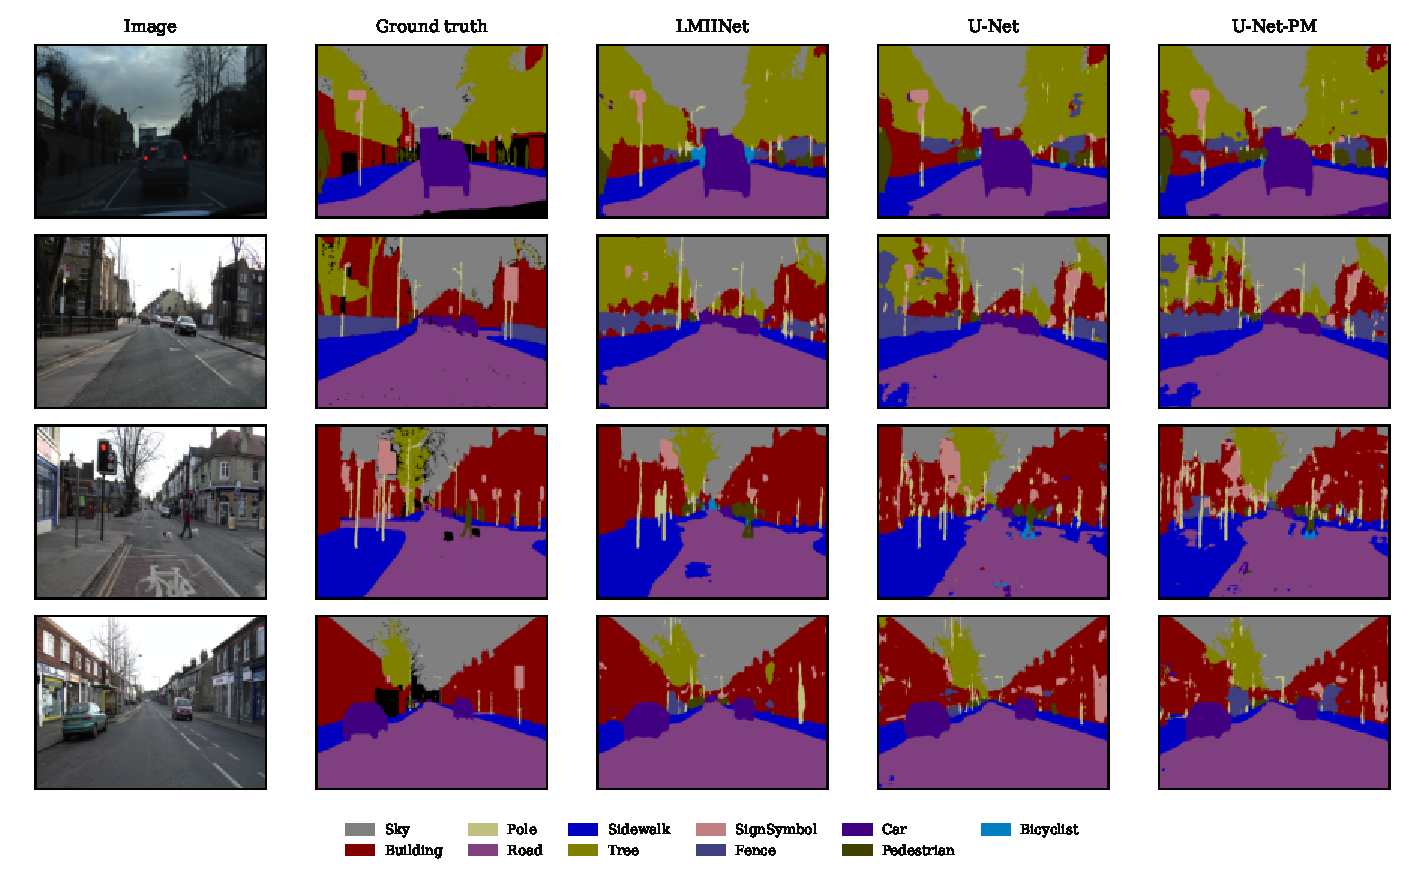
\includegraphics[width=\textwidth]{figures/04_qualitative.pdf}
\caption{CamVid test images. Columns: input, ground truth, LMIINet, U-Net, U-Net-PM.}
\label{fig:qual}
\end{figure}

Table~\ref{tab:perclass} shows where the errors are (means over three seeds). All three models
segment sky and road well, above 89\%, with sidewalk, building and tree between 67\% and 76\%. The
thin and small classes are hard for all of them: pole, sign symbol and fence lie between 17\% and
29\%, pedestrian and bicyclist between 30\% and 43\%. LMIINet's clearest gain is on bicyclist
(39.9\%, against 32.8\% for U-Net and 30.1\% for U-Net-PM), a thin class its long connections and
half-resolution head are meant to keep, and it is slightly ahead of U-Net-PM on pole and sign
symbol. The larger U-Net leads on building, tree, pedestrian and car, where its full-resolution
features and extra capacity help. LMIINet's confusion matrix (Appendix~\ref{app:curves}) shows
that most thin-class errors are pixels given to building: 34\% of sign-symbol pixels, 24\% of fence
pixels and 17\% of pole pixels. Bicyclists are confused with pedestrians (18\%) and sidewalk with
road (11\%). Pedestrian recall is 78\%, so that class's low IoU comes mostly from false positives
rather than missed people.

% =====================================================================
\section{Conclusions}
\label{sec:conclusion}
We rebuilt LMIINet from its paper with the published parameter budget and compared it with two
U-Net baselines under one recipe, one timing protocol and one GPU. Our answers to the research
questions of Section~\ref{sec:problem} are:
\begin{enumerate}
  \item[RQ1] The parameter count is reproduced (\LmiiParams{}M against 0.72M), but accuracy is not:
             \LmiiMiou\% test mIoU over three seeds against the reported 69.94\%, after about a
             twelfth of the training updates. On our laptop GPU the model runs at \LmiiFpsG{}\,FPS
             as a CUDA graph and \LmiiFps{}\,FPS in eager PyTorch.
  \item[RQ2] LMIINet is significantly less accurate than the U-Net with 2.6 times its parameters
             (1.4 points, $p = 0.04$) and on par with a U-Net of the same size (0.8 points ahead,
             not significant). It is slower than both, because its many small kernels are limited
             by launch overhead and memory traffic rather than by arithmetic.
  \item[RQ3] The Transformer, the channel reconstruction unit and the feature-enhancement decoder
             each contribute about a point. The learned interaction coefficients after which the
             network is named contribute nothing measurable, and the block's structure explains
             why: the exchange they add already happens one layer later.
  \item[RQ4] No. With half or a quarter of the training images LMIINet loses more accuracy than
             the same-size U-Net, and its small lead disappears.
\end{enumerate}
The broader lesson is that a small parameter count and MAC count do not by themselves make a fast
or a data-efficient network. Training for the paper's full schedule, more seeds for the ablations,
and timing with fused kernels on more than one device are the obvious next steps. Code, logs and
the data behind every figure are released.

\subsection{Limitations}
\label{sec:limitations}
The paper leaves the channel widths, dilation rates, form of the combination coefficients, FE
module, CAB and MLP widths and the whole training schedule unspecified. Our choices reproduce the
parameter count, but they are ours, so a gap to the paper's accuracy does not by itself show that
its numbers cannot be reproduced. We train for \Epochs{} epochs; the paper's schedule is unknown but
related work from the same group trains CamVid for about 1000 epochs~\cite{xu2023letnet}. The main
comparison uses \NumSeeds{} seeds per model, enough to show that U-Net is ahead of LMIINet
($p = 0.04$) but not to separate LMIINet from U-Net-PM. The ablations and the reduced-data study
use one seed each and are judged against the three-seed spread of the full models; the ablation
effects are consistent in direction but none is individually significant. All timings come
from one laptop GPU under Windows, and our implementation uses no fused kernels for the channel
shuffle, the CRU or the attention, which a deployment would. Finally, we evaluate on CamVid only;
Cityscapes, at four times the resolution, would test the efficiency claim harder.

\begin{ack}
This work was carried out as the course project for CSL7360 Computer Vision at IIT Jodhpur. We
received no external funding and declare no competing interests.
\end{ack}

{\small
\bibliographystyle{plainnat}
\bibliography{references}
}

% =====================================================================
\appendix

\section{Unspecified details and our choices}
\label{app:decisions}

\begin{table}[h]
\caption{Details the LMIINet paper~\cite{qiu2024lmiinet} does not give, and the choice made here.}
\centering
\scriptsize
\begin{tabular}{p{0.32\textwidth}p{0.60\textwidth}}
\toprule
Detail & Our choice \\
\midrule
Stage widths and resolutions & 32 (1/2), 64 (1/4), 128 (1/8); LETNet-style stem (three $3{\times}3$ convs, the first with stride 2) and concat(stride-2 conv, max-pool) down-sampling \\
LFIB dilation rates & encoder (1,2), (2,4), (4,8); decoder (4,2), (2,1), (1,1) \\
Combination coefficient & one learnable scalar per injection, initialised to 0.5; the right branch receives the \emph{updated} left output (Eq.~4 of the paper is ambiguous) \\
Channel shuffle groups & 2 \\
CRU hyper-parameters & SCConv defaults: split ratio 1/2, squeeze ratio 2, group convolution with 2 groups \\
FLAM & 4 heads, focusing power $p=3$, $5{\times}5$ DWC, learnable softplus scale, no positional encoding \\
Transformer depth, MLP ratio & 1 block, ratio 2 \\
CAB & compression ratio 4, channel-attention squeeze 16 \\
FE module & CBAM-style spatial gate from the semantic feature on the detail feature, then a depthwise refinement and ECA \\
Long connection & depthwise $3{\times}3$ and pointwise convolution on the encoder feature \\
SegHead & concatenation (as in the text) rather than the sum written in Eq.~13; $224\!\to\!64\!\to\!11$ channels with BN, PReLU and dropout 0.1 \\
Schedule and augmentation & \Epochs{} epochs; scale $[0.75,1.75]$, crop $360{\times}480$, flip, colour jitter \\
Class weighting & ENet weights \\
\bottomrule
\end{tabular}
\end{table}

\section{Correctness checks}
\label{app:tests}
\texttt{src/tests.py} runs before any training and the pipeline stops if one fails. Each check
compares the implementation with an independent reference; the outputs of the last run are in
\texttt{results/00\_unit\_tests.csv}.
\begin{itemize}
  \item The linear-attention product equals an explicit, row-normalised $N{\times}N$ attention
        (error $2.9{\times}10^{-7}$), and the whole FLAM module equals a slow reference written from
        the equations with the same weights (error $5.6{\times}10^{-16}$ in float64).
  \item The focusing function keeps the norm of its input and makes it more peaked.
  \item mIoU and pixel accuracy from the confusion matrix equal brute-force per-class counting with
        void pixels ignored, to $10^{-9}$.
  \item The MAC counter equals a hand count for a small network; the U-Net parameter counts equal
        a closed-form formula; LMIINet has \LmiiParams{}M parameters.
  \item Every model gives correctly shaped outputs at odd input sizes, and every parameter
        receives a gradient (which caught an auxiliary head that was not being trained in an early
        version of the test).
  \item The on-GPU augmentation reproduces the image exactly at scale 1, mirrors it exactly under
        a flip, pads with void outside the image, and never creates a label value.
  \item A training step replayed from a CUDA graph matches an eager step to within the
        run-to-run difference of two eager runs.
\end{itemize}

\section{Higher input resolution}
\label{app:hires}
The paper also reports 70.12\% mIoU at 120\,FPS for $720{\times}960$ inputs. Our
$360{\times}480$-trained LMIINet evaluated on up-sampled $720{\times}960$ inputs (labels kept at their
native resolution) reaches \LmiiMiouHiRes\% mIoU.

\begin{table}[h]
\caption{Compute and speed at $720{\times}960$ (batch 1, fp32, \BenchDevice{}).}
\centering
\small
\begin{tabular}{lcc}
\toprule
Model & GMACs & FPS (CUDA graph) \\
\midrule
\tabinput{hires_table}
\bottomrule
\end{tabular}
\end{table}

\section{Training curves and confusion matrix}
\label{app:curves}
\begin{figure}[h]
\centering
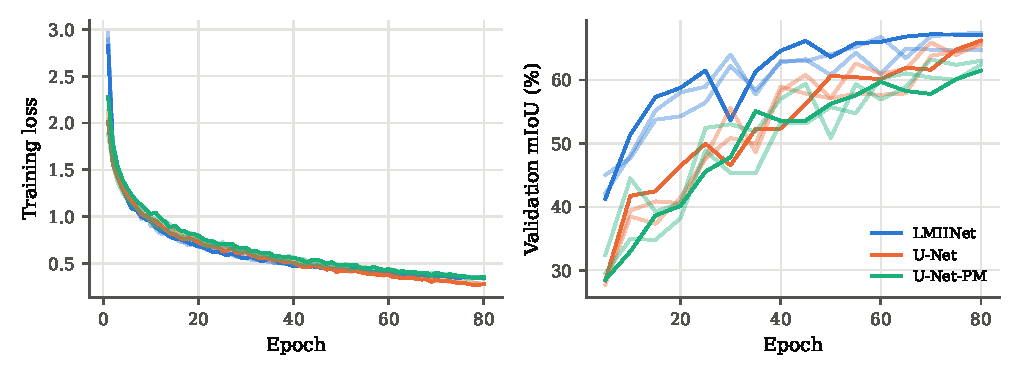
\includegraphics[width=\textwidth]{figures/03_training_curves.pdf}
\caption{Training loss and validation mIoU (every 5 epochs) of the three main models.}
\end{figure}
\begin{figure}[h]
\centering
\begin{minipage}{0.52\textwidth}\centering
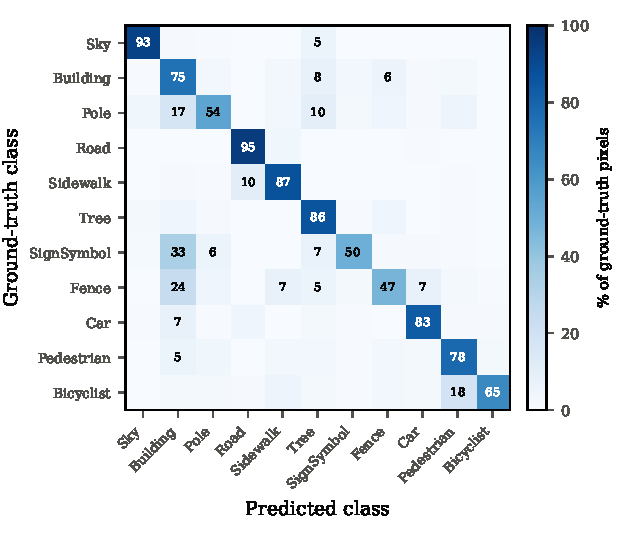
\includegraphics[width=\linewidth]{figures/06_confusion_matrix.pdf}
\end{minipage}\hfill
\begin{minipage}{0.46\textwidth}\centering
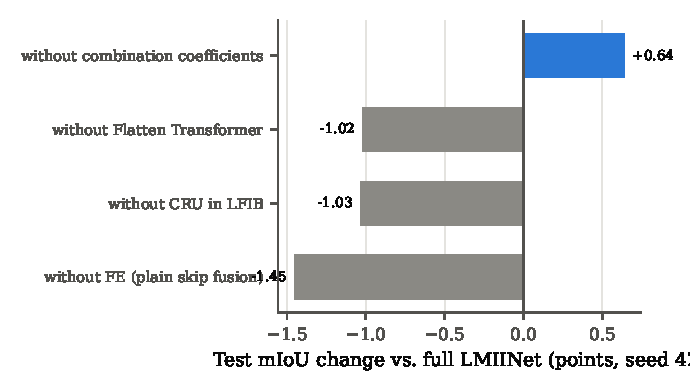
\includegraphics[width=\linewidth]{figures/07_ablation.pdf}
\end{minipage}
\caption{\textbf{Left:} row-normalised confusion matrix of LMIINet on the test set.
\textbf{Right:} change in test mIoU when one component is removed.}
\end{figure}

\section{Reproducing every number}
\label{app:repro}
\begin{verbatim}
python run.py                # everything, in order
python run.py --phase main   # one phase; finished runs are skipped
python run.py --phase main --seeds 42 7 123
\end{verbatim}
Every run is seeded; the main comparison uses seeds 42, 7 and 123 and all other runs seed 42. Code: \url{https://github.com/CoPrime69/lmiinet-camvid}.

% =====================================================================
\newpage
\section*{NeurIPS Paper Checklist}




\begin{enumerate}

\item {\bf Claims}
    \item[] Question: Do the main claims made in the abstract and introduction accurately reflect the paper's contributions and scope?
    \item[] Answer: \answerYes{} % Replace by \answerYes{}, \answerNo{}, or \answerNA{}.
    \item[] Justification: The abstract and Section~\ref{sec:intro} describe a reimplementation and small-scale reproduction; all claims are tied to the experiments in Section~\ref{sec:results}, and the reduced training budget is stated.
    \item[] Guidelines:
    \begin{itemize}
        \item The answer NA means that the abstract and introduction do not include the claims made in the paper.
        \item The abstract and/or introduction should clearly state the claims made, including the contributions made in the paper and important assumptions and limitations. A No or NA answer to this question will not be perceived well by the reviewers. 
        \item The claims made should match theoretical and experimental results, and reflect how much the results can be expected to generalize to other settings. 
        \item It is fine to include aspirational goals as motivation as long as it is clear that these goals are not attained by the paper. 
    \end{itemize}

\item {\bf Limitations}
    \item[] Question: Does the paper discuss the limitations of the work performed by the authors?
    \item[] Answer: \answerYes{} % Replace by \answerYes{}, \answerNo{}, or \answerNA{}.
    \item[] Justification: Section~\ref{sec:limitations} discusses unspecified details, the short schedule, single-device timing, seed count and the single dataset.
    \item[] Guidelines:
    \begin{itemize}
        \item The answer NA means that the paper has no limitation while the answer No means that the paper has limitations, but those are not discussed in the paper. 
        \item The authors are encouraged to create a separate "Limitations" section in their paper.
        \item The paper should point out any strong assumptions and how robust the results are to violations of these assumptions (e.g., independence assumptions, noiseless settings, model well-specification, asymptotic approximations only holding locally). The authors should reflect on how these assumptions might be violated in practice and what the implications would be.
        \item The authors should reflect on the scope of the claims made, e.g., if the approach was only tested on a few datasets or with a few runs. In general, empirical results often depend on implicit assumptions, which should be articulated.
        \item The authors should reflect on the factors that influence the performance of the approach. For example, a facial recognition algorithm may perform poorly when image resolution is low or images are taken in low lighting. Or a speech-to-text system might not be used reliably to provide closed captions for online lectures because it fails to handle technical jargon.
        \item The authors should discuss the computational efficiency of the proposed algorithms and how they scale with dataset size.
        \item If applicable, the authors should discuss possible limitations of their approach to address problems of privacy and fairness.
        \item While the authors might fear that complete honesty about limitations might be used by reviewers as grounds for rejection, a worse outcome might be that reviewers discover limitations that aren't acknowledged in the paper. The authors should use their best judgment and recognize that individual actions in favor of transparency play an important role in developing norms that preserve the integrity of the community. Reviewers will be specifically instructed to not penalize honesty concerning limitations.
    \end{itemize}

\item {\bf Theory assumptions and proofs}
    \item[] Question: For each theoretical result, does the paper provide the full set of assumptions and a complete (and correct) proof?
    \item[] Answer: \answerNA{} % Replace by \answerYes{}, \answerNo{}, or \answerNA{}.
    \item[] Justification: The paper contains no theoretical results.
    \item[] Guidelines:
    \begin{itemize}
        \item The answer NA means that the paper does not include theoretical results. 
        \item All the theorems, formulas, and proofs in the paper should be numbered and cross-referenced.
        \item All assumptions should be clearly stated or referenced in the statement of any theorems.
        \item The proofs can either appear in the main paper or the supplemental material, but if they appear in the supplemental material, the authors are encouraged to provide a short proof sketch to provide intuition. 
        \item Inversely, any informal proof provided in the core of the paper should be complemented by formal proofs provided in appendix or supplemental material.
        \item Theorems and Lemmas that the proof relies upon should be properly referenced. 
    \end{itemize}

    \item {\bf Experimental result reproducibility}
    \item[] Question: Does the paper fully disclose all the information needed to reproduce the main experimental results of the paper to the extent that it affects the main claims and/or conclusions of the paper (regardless of whether the code and data are provided or not)?
    \item[] Answer: \answerYes{} % Replace by \answerYes{}, \answerNo{}, or \answerNA{}.
    \item[] Justification: Section~\ref{sec:setup} and Appendix~\ref{app:decisions} give the full recipe and every unspecified design choice; Appendix~\ref{app:repro} lists the commands that regenerate every number.
    \item[] Guidelines:
    \begin{itemize}
        \item The answer NA means that the paper does not include experiments.
        \item If the paper includes experiments, a No answer to this question will not be perceived well by the reviewers: Making the paper reproducible is important, regardless of whether the code and data are provided or not.
        \item If the contribution is a dataset and/or model, the authors should describe the steps taken to make their results reproducible or verifiable. 
        \item Depending on the contribution, reproducibility can be accomplished in various ways. For example, if the contribution is a novel architecture, describing the architecture fully might suffice, or if the contribution is a specific model and empirical evaluation, it may be necessary to either make it possible for others to replicate the model with the same dataset, or provide access to the model. In general. releasing code and data is often one good way to accomplish this, but reproducibility can also be provided via detailed instructions for how to replicate the results, access to a hosted model (e.g., in the case of a large language model), releasing of a model checkpoint, or other means that are appropriate to the research performed.
        \item While NeurIPS does not require releasing code, the conference does require all submissions to provide some reasonable avenue for reproducibility, which may depend on the nature of the contribution. For example
        \begin{enumerate}
            \item If the contribution is primarily a new algorithm, the paper should make it clear how to reproduce that algorithm.
            \item If the contribution is primarily a new model architecture, the paper should describe the architecture clearly and fully.
            \item If the contribution is a new model (e.g., a large language model), then there should either be a way to access this model for reproducing the results or a way to reproduce the model (e.g., with an open-source dataset or instructions for how to construct the dataset).
            \item We recognize that reproducibility may be tricky in some cases, in which case authors are welcome to describe the particular way they provide for reproducibility. In the case of closed-source models, it may be that access to the model is limited in some way (e.g., to registered users), but it should be possible for other researchers to have some path to reproducing or verifying the results.
        \end{enumerate}
    \end{itemize}


\item {\bf Open access to data and code}
    \item[] Question: Does the paper provide open access to the data and code, with sufficient instructions to faithfully reproduce the main experimental results, as described in supplemental material?
    \item[] Answer: \answerYes{} % Replace by \answerYes{}, \answerNo{}, or \answerNA{}.
    \item[] Justification: The code, configurations and scripts are released (link in the abstract); CamVid is publicly available and is downloaded by \texttt{run.py}.
    \item[] Guidelines:
    \begin{itemize}
        \item The answer NA means that paper does not include experiments requiring code.
        \item Please see the NeurIPS code and data submission guidelines (\url{https://nips.cc/public/guides/CodeSubmissionPolicy}) for more details.
        \item While we encourage the release of code and data, we understand that this might not be possible, so “No” is an acceptable answer. Papers cannot be rejected simply for not including code, unless this is central to the contribution (e.g., for a new open-source benchmark).
        \item The instructions should contain the exact command and environment needed to run to reproduce the results. See the NeurIPS code and data submission guidelines (\url{https://nips.cc/public/guides/CodeSubmissionPolicy}) for more details.
        \item The authors should provide instructions on data access and preparation, including how to access the raw data, preprocessed data, intermediate data, and generated data, etc.
        \item The authors should provide scripts to reproduce all experimental results for the new proposed method and baselines. If only a subset of experiments are reproducible, they should state which ones are omitted from the script and why.
        \item At submission time, to preserve anonymity, the authors should release anonymized versions (if applicable).
        \item Providing as much information as possible in supplemental material (appended to the paper) is recommended, but including URLs to data and code is permitted.
    \end{itemize}


\item {\bf Experimental setting/details}
    \item[] Question: Does the paper specify all the training and test details (e.g., data splits, hyperparameters, how they were chosen, type of optimizer, etc.) necessary to understand the results?
    \item[] Answer: \answerYes{} % Replace by \answerYes{}, \answerNo{}, or \answerNA{}.
    \item[] Justification: Splits, optimiser, learning-rate schedule, epochs, batch size, augmentation, loss weighting and checkpoint selection are given in Section~\ref{sec:setup} and Appendix~\ref{app:decisions}.
    \item[] Guidelines:
    \begin{itemize}
        \item The answer NA means that the paper does not include experiments.
        \item The experimental setting should be presented in the core of the paper to a level of detail that is necessary to appreciate the results and make sense of them.
        \item The full details can be provided either with the code, in appendix, or as supplemental material.
    \end{itemize}

\item {\bf Experiment statistical significance}
    \item[] Question: Does the paper report error bars suitably and correctly defined or other appropriate information about the statistical significance of the experiments?
    \item[] Answer: \answerYes{} % Replace by \answerYes{}, \answerNo{}, or \answerNA{}.
    \item[] Justification: The main comparison reports the mean and sample standard deviation over three seeds and tests the differences with Welch's $t$-test (Section~\ref{sec:results}); the single-seed ablation and reduced-data runs are judged against the three-seed spread of the full models, and the text states which differences are and are not significant.
    \item[] Guidelines:
    \begin{itemize}
        \item The answer NA means that the paper does not include experiments.
        \item The authors should answer "Yes" if the results are accompanied by error bars, confidence intervals, or statistical significance tests, at least for the experiments that support the main claims of the paper.
        \item The factors of variability that the error bars are capturing should be clearly stated (for example, train/test split, initialization, random drawing of some parameter, or overall run with given experimental conditions).
        \item The method for calculating the error bars should be explained (closed form formula, call to a library function, bootstrap, etc.)
        \item The assumptions made should be given (e.g., Normally distributed errors).
        \item It should be clear whether the error bar is the standard deviation or the standard error of the mean.
        \item It is OK to report 1-sigma error bars, but one should state it. The authors should preferably report a 2-sigma error bar than state that they have a 96\% CI, if the hypothesis of Normality of errors is not verified.
        \item For asymmetric distributions, the authors should be careful not to show in tables or figures symmetric error bars that would yield results that are out of range (e.g. negative error rates).
        \item If error bars are reported in tables or plots, The authors should explain in the text how they were calculated and reference the corresponding figures or tables in the text.
    \end{itemize}

\item {\bf Experiments compute resources}
    \item[] Question: For each experiment, does the paper provide sufficient information on the computer resources (type of compute workers, memory, time of execution) needed to reproduce the experiments?
    \item[] Answer: \answerYes{} % Replace by \answerYes{}, \answerNo{}, or \answerNA{}.
    \item[] Justification: All training and timing used a single GPU (\BenchDevice); an 80-epoch LMIINet run takes \LmiiTrainMin{} minutes and a U-Net run \UnetTrainMin{} minutes on this laptop GPU (6\,GB); the full set of runs in this paper takes about four and a half GPU hours.
    \item[] Guidelines:
    \begin{itemize}
        \item The answer NA means that the paper does not include experiments.
        \item The paper should indicate the type of compute workers CPU or GPU, internal cluster, or cloud provider, including relevant memory and storage.
        \item The paper should provide the amount of compute required for each of the individual experimental runs as well as estimate the total compute. 
        \item The paper should disclose whether the full research project required more compute than the experiments reported in the paper (e.g., preliminary or failed experiments that didn't make it into the paper). 
    \end{itemize}
    
\item {\bf Code of ethics}
    \item[] Question: Does the research conducted in the paper conform, in every respect, with the NeurIPS Code of Ethics \url{https://neurips.cc/public/EthicsGuidelines}?
    \item[] Answer: \answerYes{} % Replace by \answerYes{}, \answerNo{}, or \answerNA{}.
    \item[] Justification: The work uses a public driving dataset and conforms to the NeurIPS Code of Ethics.
    \item[] Guidelines:
    \begin{itemize}
        \item The answer NA means that the authors have not reviewed the NeurIPS Code of Ethics.
        \item If the authors answer No, they should explain the special circumstances that require a deviation from the Code of Ethics.
        \item The authors should make sure to preserve anonymity (e.g., if there is a special consideration due to laws or regulations in their jurisdiction).
    \end{itemize}


\item {\bf Broader impacts}
    \item[] Question: Does the paper discuss both potential positive societal impacts and negative societal impacts of the work performed?
    \item[] Answer: \answerNA{} % Replace by \answerYes{}, \answerNo{}, or \answerNA{}.
    \item[] Justification: This is a reproduction of an existing efficient segmentation method on a public benchmark and introduces no new capability with a direct societal impact beyond that of the original work.
    \item[] Guidelines:
    \begin{itemize}
        \item The answer NA means that there is no societal impact of the work performed.
        \item If the authors answer NA or No, they should explain why their work has no societal impact or why the paper does not address societal impact.
        \item Examples of negative societal impacts include potential malicious or unintended uses (e.g., disinformation, generating fake profiles, surveillance), fairness considerations (e.g., deployment of technologies that could make decisions that unfairly impact specific groups), privacy considerations, and security considerations.
        \item The conference expects that many papers will be foundational research and not tied to particular applications, let alone deployments. However, if there is a direct path to any negative applications, the authors should point it out. For example, it is legitimate to point out that an improvement in the quality of generative models could be used to generate deepfakes for disinformation. On the other hand, it is not needed to point out that a generic algorithm for optimizing neural networks could enable people to train models that generate Deepfakes faster.
        \item The authors should consider possible harms that could arise when the technology is being used as intended and functioning correctly, harms that could arise when the technology is being used as intended but gives incorrect results, and harms following from (intentional or unintentional) misuse of the technology.
        \item If there are negative societal impacts, the authors could also discuss possible mitigation strategies (e.g., gated release of models, providing defenses in addition to attacks, mechanisms for monitoring misuse, mechanisms to monitor how a system learns from feedback over time, improving the efficiency and accessibility of ML).
    \end{itemize}
    
\item {\bf Safeguards}
    \item[] Question: Does the paper describe safeguards that have been put in place for responsible release of data or models that have a high risk for misuse (e.g., pretrained language models, image generators, or scraped datasets)?
    \item[] Answer: \answerNA{} % Replace by \answerYes{}, \answerNo{}, or \answerNA{}.
    \item[] Justification: The released models are small CamVid segmentation networks with no high risk of misuse.
    \item[] Guidelines:
    \begin{itemize}
        \item The answer NA means that the paper poses no such risks.
        \item Released models that have a high risk for misuse or dual-use should be released with necessary safeguards to allow for controlled use of the model, for example by requiring that users adhere to usage guidelines or restrictions to access the model or implementing safety filters. 
        \item Datasets that have been scraped from the Internet could pose safety risks. The authors should describe how they avoided releasing unsafe images.
        \item We recognize that providing effective safeguards is challenging, and many papers do not require this, but we encourage authors to take this into account and make a best faith effort.
    \end{itemize}

\item {\bf Licenses for existing assets}
    \item[] Question: Are the creators or original owners of assets (e.g., code, data, models), used in the paper, properly credited and are the license and terms of use explicitly mentioned and properly respected?
    \item[] Answer: \answerYes{} % Replace by \answerYes{}, \answerNo{}, or \answerNA{}.
    \item[] Justification: CamVid~\cite{brostow2009camvid} and the SegNet split~\cite{badrinarayanan2017segnet} are cited; LMIINet, FLatten Transformer, SCConv, HAT and LETNet are cited for the components we re-implement.
    \item[] Guidelines:
    \begin{itemize}
        \item The answer NA means that the paper does not use existing assets.
        \item The authors should cite the original paper that produced the code package or dataset.
        \item The authors should state which version of the asset is used and, if possible, include a URL.
        \item The name of the license (e.g., CC-BY 4.0) should be included for each asset.
        \item For scraped data from a particular source (e.g., website), the copyright and terms of service of that source should be provided.
        \item If assets are released, the license, copyright information, and terms of use in the package should be provided. For popular datasets, \url{paperswithcode.com/datasets} has curated licenses for some datasets. Their licensing guide can help determine the license of a dataset.
        \item For existing datasets that are re-packaged, both the original license and the license of the derived asset (if it has changed) should be provided.
        \item If this information is not available online, the authors are encouraged to reach out to the asset's creators.
    \end{itemize}

\item {\bf New assets}
    \item[] Question: Are new assets introduced in the paper well documented and is the documentation provided alongside the assets?
    \item[] Answer: \answerYes{} % Replace by \answerYes{}, \answerNo{}, or \answerNA{}.
    \item[] Justification: The released code is documented in its README, including usage, configuration and the list of implementation choices.
    \item[] Guidelines:
    \begin{itemize}
        \item The answer NA means that the paper does not release new assets.
        \item Researchers should communicate the details of the dataset/code/model as part of their submissions via structured templates. This includes details about training, license, limitations, etc. 
        \item The paper should discuss whether and how consent was obtained from people whose asset is used.
        \item At submission time, remember to anonymize your assets (if applicable). You can either create an anonymized URL or include an anonymized zip file.
    \end{itemize}

\item {\bf Crowdsourcing and research with human subjects}
    \item[] Question: For crowdsourcing experiments and research with human subjects, does the paper include the full text of instructions given to participants and screenshots, if applicable, as well as details about compensation (if any)? 
    \item[] Answer: \answerNA{} % Replace by \answerYes{}, \answerNo{}, or \answerNA{}.
    \item[] Justification: No crowdsourcing or human subjects were involved.
    \item[] Guidelines:
    \begin{itemize}
        \item The answer NA means that the paper does not involve crowdsourcing nor research with human subjects.
        \item Including this information in the supplemental material is fine, but if the main contribution of the paper involves human subjects, then as much detail as possible should be included in the main paper. 
        \item According to the NeurIPS Code of Ethics, workers involved in data collection, curation, or other labor should be paid at least the minimum wage in the country of the data collector. 
    \end{itemize}

\item {\bf Institutional review board (IRB) approvals or equivalent for research with human subjects}
    \item[] Question: Does the paper describe potential risks incurred by study participants, whether such risks were disclosed to the subjects, and whether Institutional Review Board (IRB) approvals (or an equivalent approval/review based on the requirements of your country or institution) were obtained?
    \item[] Answer: \answerNA{} % Replace by \answerYes{}, \answerNo{}, or \answerNA{}.
    \item[] Justification: No human subjects were involved.
    \item[] Guidelines:
    \begin{itemize}
        \item The answer NA means that the paper does not involve crowdsourcing nor research with human subjects.
        \item Depending on the country in which research is conducted, IRB approval (or equivalent) may be required for any human subjects research. If you obtained IRB approval, you should clearly state this in the paper. 
        \item We recognize that the procedures for this may vary significantly between institutions and locations, and we expect authors to adhere to the NeurIPS Code of Ethics and the guidelines for their institution. 
        \item For initial submissions, do not include any information that would break anonymity (if applicable), such as the institution conducting the review.
    \end{itemize}

\item {\bf Declaration of LLM usage}
    \item[] Question: Does the paper describe the usage of LLMs if it is an important, original, or non-standard component of the core methods in this research? Note that if the LLM is used only for writing, editing, or formatting purposes and does not impact the core methodology, scientific rigorousness, or originality of the research, declaration is not required.
    %this research? 
    \item[] Answer: \answerNA{} % Replace by \answerYes{}, \answerNo{}, or \answerNA{}.
    \item[] Justification: The core method does not use LLMs in any way; the project is a convolutional and attention-based segmentation network trained on CamVid.
    \item[] Guidelines:
    \begin{itemize}
        \item The answer NA means that the core method development in this research does not involve LLMs as any important, original, or non-standard components.
        \item Please refer to our LLM policy (\url{https://neurips.cc/Conferences/2025/LLM}) for what should or should not be described.
    \end{itemize}

\end{enumerate}




\end{document}
